\documentclass[bluish,slideColor,colorBG,pdf]{prosper}
\hypersetup{pdfpagemode=FullScreen}
\usepackage{graphicx}
\def\baselinestretch{1.0}
\setlength{\topmargin}{-60pt}
\setlength{\textheight}{460pt}
\setlength{\oddsidemargin}{0pt}
\setlength{\evensidemargin}{0pt}
\setlength{\textwidth}{660pt}
\setlength{\footskip}{0pt}
\parindent 0.3in
\hyphenpenalty=10000
\tolerance=10000
\pagestyle{empty}

\def\Prob{{\rm Prob\;}}
\def\prob{{\rm \;Prob\;}}


\author{January 2017}
\title{Genome 562}
\institution{Week 1}

\begin{document}

\maketitle

\begin{slide}[Replace]{Early workers in theoretical population genetics}
\vspace{0.5in}

\begin{center}
\begin{tabular}{c c c}
\includegraphics[height=1.3in]{Castle.ps} &
\includegraphics[height=1.3in]{Yule.ps} &
\includegraphics[height=1.3in]{Punnett.ps}\\
& & \\
William Ernest Castle & G. Udny Yule & R. C. Punnett\\
\vspace{0.1in}
1867 -- 1962 & 1871 -- 1951 & 1875 -- 1967
\end{tabular}
\end{center}

\end{slide}

\begin{slide}[Replace]{Godfrey Harold Hardy (1877 - 1947) }

\centerline{\includegraphics[width=1.8in]{hardy.ps}}

\end{slide}

\begin{slide}[Replace]{Wilhelm Weinberg (1862 - 1937) }
\bigskip

\centerline{\includegraphics[width=1.5in]{weinberg.ps}}

\end{slide}

\begin{slide}[Replace]{Fleeming Jenkin (1833 - 1885) }

\centerline{\includegraphics[width=2.0in]{jenkin1.ps}}

\end{slide}

\begin{slide}[Replace]{Herbert S. Jennings (1868 - 1947) }
\bigskip

\centerline{\includegraphics[width=2.0in]{jennings.ps}}

\end{slide}

\end{document}
